\documentclass[12pt]{article}
\usepackage[utf8]{inputenc}
\usepackage{enumerate}
\usepackage{amsmath}
\usepackage{graphicx}
\usepackage{subfig}
\usepackage{caption}
\usepackage{hyperref}
\usepackage{wrapfig}
\usepackage{rotating}
\usepackage{pdflscape}
\usepackage[left=2cm, right=2cm, top=2cm,bottom=2cm]{geometry}
\usepackage[framed,numbered,autolinebreaks,useliterate]{mcode}

\title{AAE550: HW2}
\author{Rahul Deshmukh \\\href{mailto:deshmuk5@purdue.edu}{{\color{blue}deshmuk5@purdue.edu}} \\\texttt{PUID: 0030004932}}
\date{\today}
\begin{document}
\maketitle
\begin{enumerate}[I]
\item \underline{\textbf{Constrained Minimization in N variable- Direct Methods}}\\
%explanation of problem
For this homework we are required to carry out constrained minimization using different direct methods (SLP/MOC,GRG,SQP) to find out the optimized configuration of support column for a sign.\\

We are presented with the geometry of the sign post as shown in figure \ref{fig:main_fig}. The height to the bottom of the sign \textbf{H}, the width of the sign \textbf{b}, and the wind pressure \textbf{p} on the sign are as follows: $H= 20$ m , $b=8$ m , $p=900$ N/m . The weight of the sign per unit area, \textbf{w}, is 2.9 kN/m . It is required to find the column base diameter, \textbf{$d_0$}, and thickness, \textbf{t}, to \textit{minimize} the \textit{mass of the column}. The predetermined height of the sign, \textbf{h}, is 4.00 [m].\\

Material properties for the column is given as the Young's Modulus as $E=79$ GPa and the density as $\rho=2300$ Kg/$m^3$
% problem fig
\begin{figure}[!h]
  \centering
    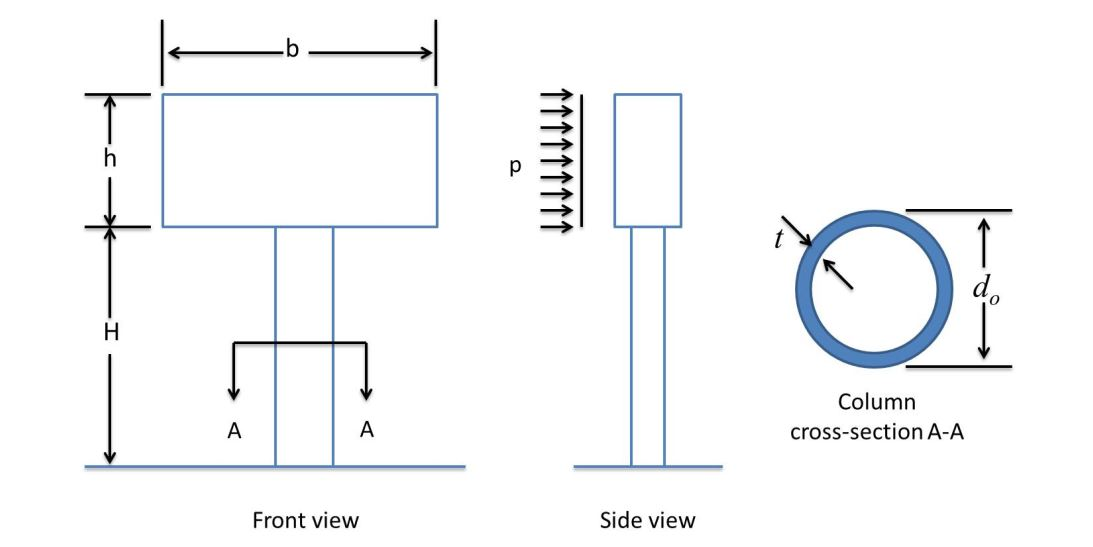
\includegraphics[width=0.8\textwidth]{problem_fig.JPG}
    \caption{Geometry of problem}
  \label{fig:main_fig}
\end{figure}

The constraints for the design of the column dictate that, The column must be safe with respect to axial stress, bending stress, local buckling and the deflection of sign, $\delta$ must not exceed $0.1$ m. For this problem, The allowable axial stress if given by $\sigma_a=300$ MPa and the allowable bending stress in the column is $\sigma_{b}=140 $ MPa. Further, to prevent local buckling of the column, the diameter to thickness ratio, $d_0$/t, must not exceed $90$.\\

Also, In addition to the above design constraints we can anticipate another geometric constraint, that the inner diameter of the column should be greater than or equal to 0. To put it mathematically we can say that $d_0-2t\geq0$.\\

We can now proceed with formulating our minimization problem with the help of formulas for axial stress, bending stress, $\delta$ as given in the problem description.\\

It is to be \textbf{noted} that I will be using standard \textbf{SI units (MKS)} for all of the quantities. The bounds for the variables $d_0$ and t as given in the problem description are in cms and will be needed to be changed to m.\\

\begin{enumerate}[1)]
    \item Optimization Problem Statement:\\
    
    For this problem, I have chosen my design variables $\vec{x}$ as the variables $d_0$ and t itself.\\ 
    
    \textbf{Note:} I observed that when choosing certain variable transformations, I was getting simplified objective function and even some constraints got simplified, but the transformations resulted in making some of my constraints more complicated resulting in even more complex analytical derivatives.\\
    
    I tried to formulate the problem with the following transformations:\\
    \begin{enumerate}[i)]
        \item Using $\vec{x}^T = \begin{bmatrix} d_0/t& 1/t \end{bmatrix}$
        \item Using $\vec{x}^T = \begin{bmatrix} d_0^2-(d_0-2t)^2 & d_0^2+(d_0-2t)^2 \end{bmatrix}$
        \item Using $\vec{x}^T = \begin{bmatrix}  ((250-10)d_0+10)/100 & ((10-0.05)t+0.05)/100\end{bmatrix}$ (to bring to the variables to the range of 0-1)
    \end{enumerate}
    For all of these Transformation I observed that, I was not able to obtain a total win-win transformation which will simplify all the constraints and objective function. Therefore, I chose the option of choosing my design variables as the original variables.\\
    
    I obtained my objective function and constraints using symbolics in matlab, The script for this task is as follows:
    \begin{lstlisting}
    % Homwwork 2 
% symbolics for obj fun and constraints
% Rahul Deshmukh
% PUID: 0030004932
% deshmuk5@purdue.edu
%%
clc; clear all;
format long;

% define constants
H=20; % m
b=8; % m
p=900; %Pa
h=4; % m
w=2.9E3; % N/m^2
E=79E9; % Pa
rho=2300; %kg/m^3 
% bounds
s_ax_ub=300E6; %Pa
s_ben_ub=140E6; %Pa
del_ub=0.1;  %m
%%

%define symbolics for d0 ant t
syms d0 t;
% derived constants
F=p*b*h; % total wind force in N
W=w*b*h; % total weight in N

A=pi/4*(d0^2-(d0-2*t)^2);% area of crossection
I=pi/64*(d0^4-(d0-2*t)^4);% moment of inertia

del=(F/(E*I))*(H^3/3+H^2*h/2+H*h^2/4) % deflection
M= W*del; % moment

s_ax= W/A; % axial stress
fprintf('s_ax');
vpa(s_ax)

s_ben=M*d0/(2*I); % bending stress
fprintf('s_ben');
vpa(s_ben)


vol= pi*(d0^2-(d0-2*t)^2)/4*H

% gradients of obj fun and constraints
% grad obj
fprintf('grad f');
gradient(vol,[d0,t])

%gradient axial stress
fprintf('grad s_ax')
gradient(s_ax,[d0,t])

%gradient bending stress
fprintf('grad s_ben')
gradient(s_ben,[d0,t])

%gradient deflection
fprintf('grad del')
gradient(del,[d0,t])

fprintf('----------------simplified constraints-------------\n');
%s_ax
g1=simplify(118156.62975142309727481930592775/s_ax_ub+(1.0*(d0 - 2.0*t)^2 - d0^2))
gradient(g1,[d0,t])
% s_ben
g2=simplify((24897.970775523786790537249623513*d0)/s_ben_ub-(1.0*(d0 - 2.0*t)^4 - d0^4)^2)
gradient(g2,[d0,t])
%del
g3=simplify(102144/del_ub-(1234375*pi*(d0^4 - (d0 - 2*t)^4)))
gradient(g3,[d0,t])
% d0/t ratio
g4=d0-90*t
gradient(g4,[d0,t])
% geometric constraint
g5=2*t-d0
gradient(g5,[d0,t])

fprintf('--------------------- in x1 and x2------------------------\n');
% change to x1 and x2
syms x1 x2;
%scaling
% t1=(240*x1+10)/100;
% t2=(((10-0.05)*x2)+0.05)/100;
% transformation
t1=x1/x2;
t2=1/x2;
% t1=((x1+x2)/2)^0.5;
% t2=(t1-( ((x2-x1)/2)^0.5 ))/2;

fprintf('axial stress');
s_ax=vpa(simplify(subs(s_ax,[d0,t],[t1,t2]))) 
% (29539.157437855774318704826481939*x2^2)/(x1 - 1.0)
% comment 2<x1<=90 so denominator is never zero

fprintf('bending stress');
s_ben=vpa(simplify(subs(s_ben,[d0,t],[t1,t2])))
% (389.0307933675591686021445253674*x1*x2^7)/(x1^3 - 3.0*x1^2 + 4.0*x1 - 2.0)^2
% roots([1,-2,4,-2]) are all imaginary numbers: so denominator never zero

fprintf('deflection');
del=vpa(simplify(subs(del,[d0,t],[t1,t2])))
% (0.0032925007609475558839041748103133*x2^4)/(x1^3 - 3.0*x1^2 + 4.0*x1 - 2.0)

fprintf('volume obj');
vol=vpa(simplify(subs(vol,[d0,t],[t1,t2])))

% gradients of obj fun and constraints
% grad obj
fprintf('grad f');
gradient(vol,[x1,x2])

%gradient axial stress
fprintf('grad s_ax')
gradient(s_ax,[x1,x2])

%gradient bending stress
fprintf('grad s_ben')
gradient(s_ben,[x1,x2])

%gradient deflection
fprintf('grad del')
gradient(del,[x1,x2])
    \end{lstlisting}
    
    The Optimization problem for $\vec{x}^T=\begin{bmatrix}d_0 & t\end{bmatrix}$then becomes:\\
    \begin{enumerate}[a)]
        \item Objective function f(x)\\
        As we are required to minimize the mass of the cylindrical column in this problem. The Mass of the column is given as $\rho*Volume$ as $\rho$ here is a constant. Therefore, for our minimization problem we can remove the constant $\rho$ and just minimize the Volume ($\pi*(d_0^2-(d_0-2t)^2)/4*H$). The objective function in terms of the design variables is:\\
    $$\min_{\vec{x}} f(x)= 5\pi(x_1^2 - (x_1 - 2x_2)^2) [m^3]$$
    
    And the analytical gradient is given by:\\
$\nabla f(x) = \begin{bmatrix} 20\pi x_2\\ 5\pi(4x_1 - 8x_2) \end{bmatrix}$ [$m^2$]\\
    
        \item Inequality Constraints ($g_j(x)$):
        \begin{enumerate}[i)]
            \item Constraint on Axial Stress (\textbf{Non-Linear Constraint}) \\
$$\sigma_{axial}=W/A\leq \sigma_a $$
$$\Rightarrow118156.62975142309727481930592775/(x_1^2-(x_1 - 2x_2)^2)\leq300E6$$
$$\Rightarrow118156.62975142309727481930592775/300E6 \leq(x_1^2-(x_1 - 2x_2)^2)$$
$$\Rightarrow g_1(x)=4x_2^2 - 4x_1x_2 + 908168795681899/2305843009213693952 [m^2]$$

And the analytical gradient is given by:\\
$\nabla g_1(x) = \begin{bmatrix}-4x_2\\ 8x_2-4x_1 \end{bmatrix}$ [m]\\

            \item Constraint on Bending Stress (\textbf{Non-Linear Constraint})\\
$$\sigma_{bending}=\frac{M}{2I}d_0 \leq \sigma_b$$
$$\Rightarrow  (24897.970775523786790537249623513x_1)/((x_1 - 2x_2)^4 - x_1^4)^2\leq 140E6$$
$$\Rightarrow  (24897.970775523786790537249623513x_1)/140E6 \leq ((x_1 - 2x_2)^4 - x_1^4)^2$$
$$\Rightarrow g_2(x)= (6843902093928859*x_1)/38482906972160000000 - (x_1^4 - (x_1 - 2x_2)^4)^2[m^8]$$

And the analytical gradient is given by:\\
$\nabla g_2(x) = [6843902093928859/38482906972160000000 - 2(x_1^4 - (x_1 - 2*x_2)^4)(4x_1^3 - 4(x_1 - 2x_2)^3)$\textbf{,}$
-16(x_1^4 - (x_1 - 2x_2)^4)(x_1 - 2x_2)^3]
$ [$m^7$]\\


    \item Constraint on deflection (\textbf{Non-Linear Constraint})\\
$$\delta\leq0.1[m]$$
$$\Rightarrow 102144/(1234375\pi(x_1^4 - (x_1 - 2x_2)^4))\leq 0.1$$
$$\Rightarrow 102144/0.1 \leq (1234375\pi(x_1^4 - (x_1 - 2x_2)^4)) $$
$\Rightarrow g_3(x)= (8327734208259683(x_1 - 2x_2)^4)/2147483648 - (8327734208259683x_1^4)/2147483648 + 1021440 [m^4]$\\

And the analytical gradient is given by:\\
$\nabla g_3(x) = \begin{bmatrix}
(8327734208259683(x_1 - 2x_2)^3)/536870912 - (8327734208259683x_1^3)/536870912\\
-(8327734208259683(x_1 - 2x_2)^3)/268435456
\end{bmatrix}
$ [$m^3$]\\

\item Constraint for Buckling (\textbf{Linear Constraint})\\
$$d_0/t\leq90$$
$$\Rightarrow x_1/x_2\leq90$$
$$\Rightarrow x_1\leq90x_2$$
$$\Rightarrow g_4(x)=x_1- 90x_2\leq0 [m]$$

The analytical gradient is given by:\\
$\nabla g_4(x) = \begin{bmatrix}
1\\
-90
\end{bmatrix}
$ [No units]\\

\item Geometric Constraint (\textbf{Linear Constraint})\\
$$d_0-2t\geq0$$
$$\Rightarrow x_1-2x_2\geq0$$
$$\Rightarrow g_5(x)=2x_2-x_1\leq0[m]$$

The analytical gradient is given by:\\
$\nabla g_4(x) = \begin{bmatrix}
-1\\
2
\end{bmatrix}
$ [No units]\\

\end{enumerate}%[i)]
\textbf{Note}: For all of the above constraints I am taking the expression in the denominator to the RHS so that my final expression for the constraint will not contain any design variables in the denominator. This helps in getting simpler analytical derivatives and as we will be using LP/QP solvers, it is best to not have the design variables in the denominator because otherwise our linear approximation of the gradient will no longer hold true.\\

\newpage
            \item Design variable Bounds\\
\begin{enumerate}[i)]
    \item Bounds on $d_0$\\
    $$10/100\leq d_0\leq250/100 [m]$$
    $$\Rightarrow 10/100\leq x_1\leq250/100 [m]$$
    \item Bounds on t\\
    $$0.05/100\leq t \leq10/100 [m]$$
    $$\Rightarrow 0.05/100\leq x_2 \leq10/100 [m]$$
\end{enumerate}

\textbf{Note:} Bounds will be treated as constraints for GRG solver in Excel. For the rest of methods ie SLP,MOC,SQP the bounds will be handled directly.
    \end{enumerate}%[a)]

\newpage    
\item Solving the optimal design of the column using one of the two methods which use LP:\\

For this task I have chosen the \textbf{Methods of Centers} for finding the optimal solution. As our design variables have different order of magnitudes for the bounds, I am choosing the move limits such that the move made is of the same percentage in the \textit{domain} of the design variables. For my code I am using p=5\% as the move limit. The move limits for ($x_1$,$x_2$) in the code will then become Delta\_x=(p/100)*(ub-lb)= (0.1200[m],0.0050 [m]), where \textbf{ub} and \textbf{lb} will be the vectors for the upper bound and lower bounds of the design variables.\\

Also, I am taking a uniform value of $10^{-4}$ the tolerance for change in objective function, change in inequality constraints. 

Matlab code for this task is as follows:\\

The code for defining Objective function:
\begin{lstlisting}
function [f, grad_f] = example_fun(x)
% Homework 2 
% Rahul Deshmukh
% PUID: 0030004932
% obj function 
%%
% obj is to reduce the total volume
f = 5*pi*(x(1)^2 - (x(1) - 2*x(2))^2) ;% pi*(d0^2-(d0-x(2))^2)/4*H    

if nargout > 1  % fun called with two output arguments
    % Matlab naming convention will use grad_f(1) as df/dx(1); 
    % grad_f(2) as df/dx(2)
    grad_f = [20*pi*x(2);... 
               5*pi*(4*x(1) - 8*x(2))];      % Compute the gradient evaluated at x
end
\end{lstlisting}

The code for defining the Constraints:
\begin{lstlisting}
function [g, h, grad_g, grad_h] = example_con(x)
% the format used here is compatible with fmincon
% non-linear constraint functions 
% Homework 2 
% Rahul Deshmukh
% PUID: 0030004932
%%
% constants
s_ax_ub=300E6; %Pa
s_ben_ub=140E6; %Pa
del_ub=0.1; %m

%%
% inequality constraints
g(1) = 4*x(2)^2 - 4*x(1)*x(2) + 908168795681899/2305843009213693952; %s_ax
g(2) = (6843902093928859*x(1))/38482906972160000000 - (x(1)^4 - (x(1) - 2*x(2))^4)^2; %s_ben
g(3) = (8327734208259683*(x(1) - 2*x(2))^4)/2147483648 - (8327734208259683*x(1)^4)/2147483648 + 1021440; % del
g(4) = x(1)-90*x(2); % d0/t < 90
g(5) = 2*x(2)-x(1); % geometric constraint

%%
% equality constraints - none in this problem
h = [];

% compute gradients
if nargout > 2   % called with 4 outputs
    % Matlab naming convention uses columns of grad_g for each gradient
    % vector. 
    grad_g=[];
    grad_g = [grad_g,[-4*x(2);...
                       8*x(2) - 4*x(1)]]; % s_ax
                  
    grad_g=[grad_g,[ 6843902093928859/38482906972160000000 - 2*(x(1)^4 - (x(1) - 2*x(2))^4)*(4*x(1)^3 - 4*(x(1) - 2*x(2))^3);....
                    -16*(x(1)^4 - (x(1) - 2*x(2))^4)*(x(1) - 2*x(2))^3 ]];% s_ben       
               
    grad_g=[grad_g,[(8327734208259683*(x(1) - 2*x(2))^3)/536870912 - (8327734208259683*x(1)^3)/536870912;...
                    -(8327734208259683*(x(1) - 2*x(2))^3)/268435456]];% del            
                 
    grad_g=[grad_g,[1;-90]]; % d0/t < 90
    grad_g=[grad_g,[-1;2]]; % d0 - 2*t > 0
    grad_h = [];    % no equality constraints
end
end
\end{lstlisting}

The main code for MOC is:
\begin{lstlisting}
%  written with MATLAB 2018a
clc;clear all;
% convergence tolerance for change in function value between minimizations
epsilon_f = 1e-04;
% convergence tolerance for maximum inequality constraint value
epsilon_g = 1e-04;
% convergence tolerance for maximum equality constraint violation
epsilon_h = 1e-04;
% stopping criterion for maximum number of sequential minimizations
max_ii = 50;

% set options for linprog to use medium-scale algorithm
% also suppress display during loops
options = optimoptions('linprog','Algorithm','dual-simplex','Display','iter');

% design variables:
% x0 = [(250+10)/2;(0.05+10)/2 ]/100;% initial design point 
x0=[100;8]/100;
% account for number of design variables
n = length(x0);
% lower bounds from original problem - must enter values, use -Inf if none
lb = [10;0.05]/100;
% upper bounds from original problem - must enter values, use Inf if none
ub = [250;10]/100
% delta x values for move limits
p=5; % percentage of length of any dim
Delta_x = (p/100)*(ub-lb); % same percentage move in all dims

% initial objective function and gradients
[f,gradf] = example_fun(x0);

% constraints of centers problem use gradients of objective and
% constraints and values of the constraint functions
[g, h, gradg, gradh] = example_con(x0);

f_last = 1e+5;       % set first value of f_last to large number
ii = 0;              % set counter to zero
fprintf('#-----------------start--------------------------#\n');
while (((abs(f_last - f) >= epsilon_f) | (max(g) >= epsilon_g)) ...
        & (ii < max_ii))
    % increment counter
    ii = ii + 1   % no semi-colon to obtain output

    % store 'f_last' value
    f_last = f;
    
    % first approximation uses information from gradients of the objective
    % function and constraint functions to build the problem that searches
    % for the center of the hypersphere
    % objective of the hypersphere problem is to minimize -r (biggest
    % radius) 'linprog' uses coefficients of objective as input
    fcoeff = [zeros(n,1); -1];

    % first constraint for method of centers uses tangent to constant f(x);
    % remaining i through m constraints use tangent to g(x) = 0
    % for linprog, these linear constraints are entered using A * x <= b 
    % format first row of A is usability related constraint; first n 
    % columns are elements of gradf, n+1 column is norm of gradf
    use_A = [gradf', norm(gradf)];
    
    % remaining rows of A are feasibility related constraints; first n
    % columns are elements of gradg_j, n+1 column are norm of gradg_j
    colnormg = sqrt(sum(gradg.^2,1)); % 2-norm of each column in gradg
    feas_A = horzcat(gradg', colnormg');
    
    % check for infeasible initial design; if infeasible omit
    % usability constraint from LP problem
    if max(g) > 0
        A = feas_A;
        b = -g';
    else
        A = vertcat(use_A, feas_A);
        b = [0; -g'];
    end
    
    A = vertcat(use_A, feas_A);
    b = [0; -g'];
    
    % the MoC LP has no equality constraints
    Aeq = [];
    beq = [];
    
    % search variables for method of centers
    % s(1:n) used for update; s(n+1) = radius
    % initial guess and move limits
    s0 = zeros(n+1,1);
    % move limits on LP problem (see slide 23-26 from class 17)
    % combines original problem bounds on x with move limits
    % this keeps s values within move limits on x, and allows for
    % positive radius on hypersphere.  No upper bound needed for r,
    % so use Inf
    lb_LP = [max(-1*Delta_x, (lb - x0)); 0];      
    ub_LP = [min(Delta_x, (ub - x0)); Inf];      
    
    [s,radius,exitflag] = linprog(fcoeff,A,b,Aeq,beq,lb_LP,ub_LP,options);
    
    % This will only provide the search direction vector and the value of
    % the hypersphere radius.  Use update formula to find next x; then
    % compute new functions values, store x as new x0, increment counter
    % note:  the s vector here has n+1 elements; to update x, we only need 
    % s(1:n), s(n+1) is radius
    x = x0 + s(1:n)  % no semi-colon to obtain output
    [f,gradf] = example_fun(x);
    f   % no semi-colon to obtain output
    [g, h, gradg, gradh] = example_con(x);
    g   % no semi-colon to obtain output
    x0 = x;
    fprintf('#----------------------------------------------------------#\n');
end
exitflag
fprintf(strcat('Total iters: ',num2str(ii),'\n'));
\end{lstlisting}

\newpage
%table for MOC
Summary table for MOC:\\

\begin{tabular}{|c|c|c|c|c|c|c|c|}
\hline 
MOC &	Run 1 &	Run 2\\
\hline
x0 [m]&	1.3&	1\\

	&0.05025&   0.08\\
\hline	
x* [m]&	1.32302415291342&	1.323024152659610\\
% \hline
	&0.01470115530768&	0.014701133292546\\
\hline
f(x*) [$m^3$]&	1.2084990392&	1.2084972495\\
\hline
g1(x) [$m^2$]&	-0.0765415829&	-0.076541469\\
% \hline
g2(x) [$m^8$]	&-0.0691523985&	-0.0691521976\\
% \hline
g3(x) [$m^4$]&	-59.5989631545&	-58.1198377907\\
% \hline	
g4(x) [m]	&-7.98247780400274E-005&	-7.78436695543228E-005\\
% \hline
g5(x) [m]	&-1.2936218423&	-1.2936218861\\
\hline
num iters&	18&	24\\
\hline
exitflag&	1&	1\\
\hline
\end{tabular}\\


\item Solving the problem using Generalized Reduced Gradient (GRG) Nonlinear method in Excel solver\\

\textbf{Note}: The bounds for the design variables were entered as constraints for the excel solver. For more details, please refer to figures \ref{fig:excel formulas}(for cell references) and figure \ref{fig: excel solver option}(for solver parameters). Also, the excel solver will be using Numerical derivatives for the GRG solver, in my case I am using \textbf{Central differences} to find the derivatives (this can also be verified in answer report screen shots).\\

I ran the GRG solver for two different initial solutions:\\

$x0=\begin{bmatrix} 1.3\\ 0.0525\end{bmatrix}$ and $x0=\begin{bmatrix} 1\\ 0.08\end{bmatrix}$

The screen shot of different worksheets is as follows:\\
\newpage
\begin{figure}[!hp]
  \centering
    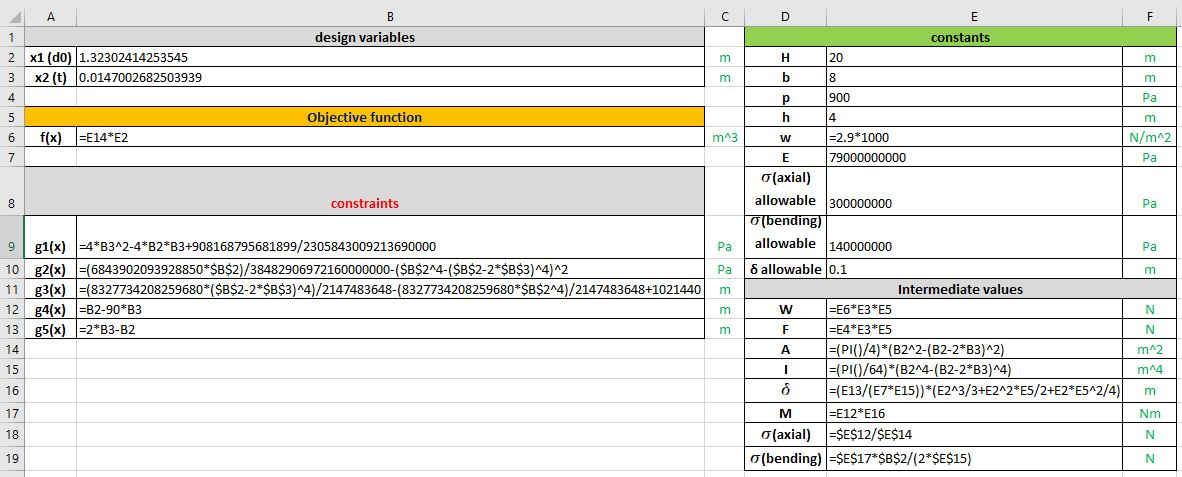
\includegraphics[angle=90,width=0.5\textwidth]{formulas.JPG}
  \caption{Problem setup: worksheet with formulas}
  \label{fig:excel formulas}
\end{figure}
\begin{figure}[!hp]
  \centering
    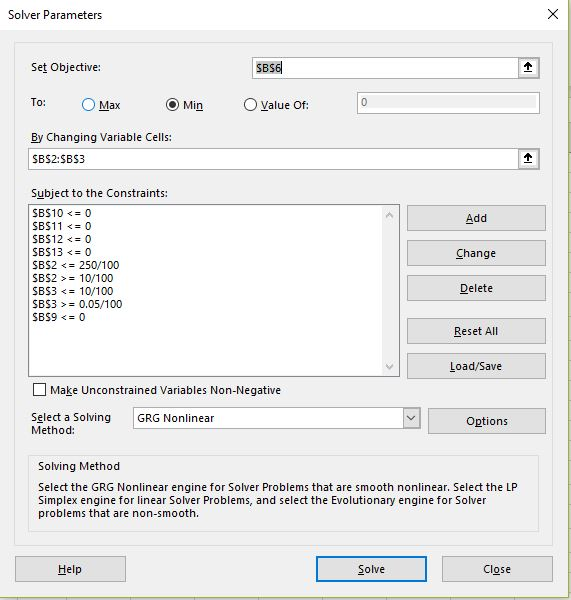
\includegraphics[width=0.9\textwidth]{solver.JPG}
  \caption{Problem setup: Solver options}
  \label{fig: excel solver option}
\end{figure}
\newpage
\begin{figure}[!hp]
  \centering
    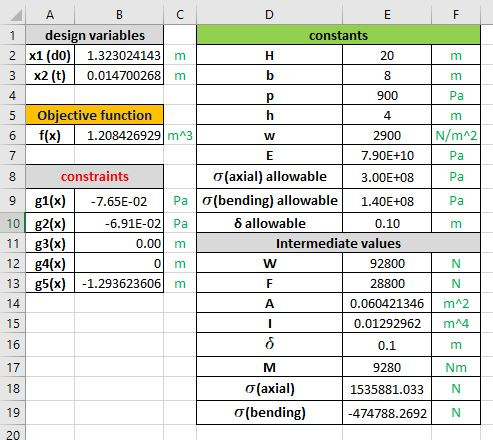
\includegraphics[width=0.8\textwidth]{after.JPG}
  \caption{Problem setup after running the solver}
\end{figure}
\begin{figure}[!htbp]
    \subfigure{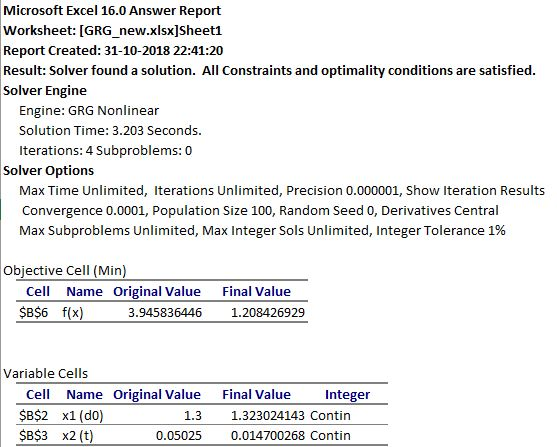
\includegraphics[width=0.8\textwidth]{ans1_1.JPG}}
    \subfigure{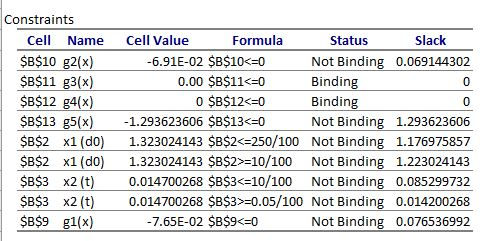
\includegraphics[width=0.6\textwidth]{ans1_2.JPG}}
    \caption{Answer report for run 1}
\end{figure}
\begin{figure}[!htbp]
  \centering
    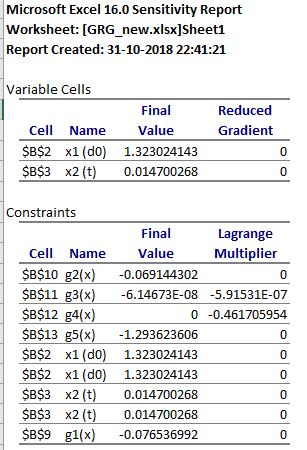
\includegraphics[width=0.5\textwidth]{sens1.JPG}
  \caption{Sensitivity Report for run 1}
\end{figure}
\begin{figure}[!htbp]
    \subfigure{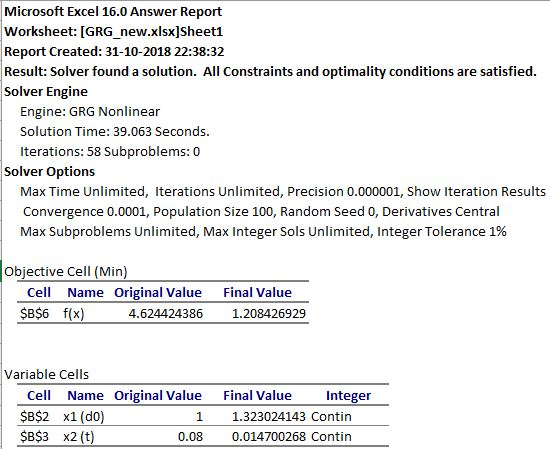
\includegraphics[width=0.8\textwidth]{ans2_1.JPG}}
    \subfigure{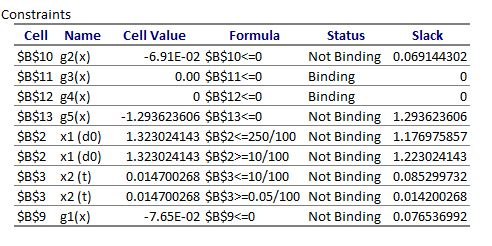
\includegraphics[width=0.6\textwidth]{ans2_2.JPG}}
    \caption{Answer report for run 2}
\end{figure}
\begin{figure}[!htbp]
  \centering
    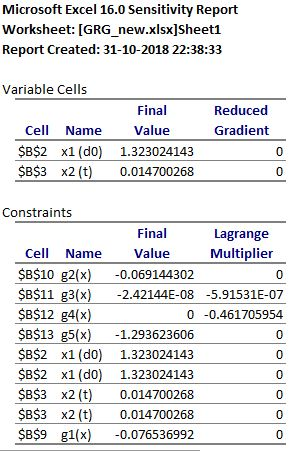
\includegraphics[width=0.5\textwidth]{sens2.JPG}
  \caption{Sensitivity Report for run 2}
\end{figure}

\newpage
Summary Table for GRG is:\\
\begin{tabular}{|c|c|c|c|c|c|c|c|}
\hline 
GRG &	Run 1 &	Run 2\\
\hline
x0 [m]&	1.3&	1\\

	&0.05025&   0.08\\
\hline	
x* [m]&	1.3230241425&	1.3230241425\\
% \hline
	&0.0147002683 &	0.0147002683\\
\hline
f(x*) [$m^3$]&	1.208427107&	1.2084269289\\
\hline
g1(x) [$m^2$]&	-7.65E-02 &	-7.65E-02\\
% \hline
g2(x) [$m^8$]	&-6.91E-02&	-6.91E-02\\
% \hline
g3(x) [$m^4$]&	0.00&	0.0\\
% \hline	
g4(x) [m]	&4.81170658872543E-013&	0\\
% \hline
g5(x) [m]	&-1.293623606&	-1.293623606\\
\hline
num iters&	4&	58\\
\hline
exitflag&	$1^*$&	$1^*$\\
\hline
\end{tabular}\\
value of 1* for exitflag in the summary table for GRG refers to the exit message by the solver: \textbf{'Solver found a solution.  All Constraints and optimality conditions are satisfied'}\\

\textbf{Comment:} I was curious as to what would be the performance of GRG solver with original set of equations for constraints (ie without taking the denominator to the RHS) that makes the whole optimization problem in terms of $\vec{x}=$[$d_0$ t]:\\
$$\min_{\vec{x}} f(x)= 5\pi(x_1^2 - (x_1 - 2x_2)^2) [m^3]$$
$$g_1(x)=\frac{W}{((\pi/4)*(x_1^2-(x_1-2x_2)^2))} [Pa]$$
$$g_2(x)=\frac{(M*x_1)}{(2*((\pi/64)*(x_1^4-(x_1-2x_2)^4)))} [Pa]$$
$$g_3(x)=\delta=\frac{\pi}{64}*(x_1^4-(x_1-2x_2)^4)[m]$$
$$g_4(x)=x_1-90x_2 [m]$$
$$g_5(x)=2x_2 -x_1[m]$$
Where $W=wbh$ and $M=W\delta$\\

In this case I was getting the same optimal solution but with only 6 and 9 number of iterations for runs 1 and 2 respectively. However, for the sake of uniformity for comparison of results I will not be reporting the screen-shots/summary table for this case.

\newpage
\item Solving the problem with Sequential Quadratic Programming (SQP) method with numerical gradients:\\

For efficient performance of SQP we split the constraints into two categories: Linear and Non-Linear Constraints and then give them as inputs to the \textit{fmincon} function in matlab.\\

The Matlab scripts are as follows:\\
The code for objective function (remains unchanged: same as that for MOC)
\begin{lstlisting}
function [f, grad_f] = example_fun(x)
% Homework 2 
% Rahul Deshmukh
% PUID: 0030004932
% obj function 
%%
% obj is to reduce the total volume
f = 5*pi*(x(1)^2 - (x(1) - 2*x(2))^2) ;% pi*(d0^2-(d0-x(2))^2)/4*H    

if nargout > 1  % fun called with two output arguments
    % Matlab naming convention will use grad_f(1) as df/dx(1); 
    % grad_f(2) as df/dx(2)
    grad_f = [20*pi*x(2);... 
               5*pi*(4*x(1) - 8*x(2))];      % Compute the gradient evaluated at x
end
\end{lstlisting}
The code for Non-Linear Constraints:
\begin{lstlisting}
function [g,h,grad_g,grad_h]=sqp_con(x)

%%
% Non-Linear inequality constraints
g(1) = 4*x(2)^2 - 4*x(1)*x(2) + 908168795681899/2305843009213693952;
g(2) = (6843902093928859*x(1))/38482906972160000000 - (x(1)^4 - (x(1) - 2*x(2))^4)^2;
g(3) = (8327734208259683*(x(1) - 2*x(2))^4)/2147483648 - (8327734208259683*x(1)^4)/2147483648 + 1021440;

%%
% equality constraints - none in this problem
h = [];

% compute gradients
if nargout > 2   % called with 4 outputs
    % Matlab naming convention uses columns of grad_g for each gradient
    % vector. 
    grad_g=[];
    
    % s_ax
    grad_g = [grad_g,[-4*x(2);...
                       8*x(2) - 4*x(1)]]; 
    % s_ben
    grad_g=[grad_g,[ 6843902093928859/38482906972160000000 - 2*(x(1)^4 - (x(1) - 2*x(2))^4)*(4*x(1)^3 - 4*(x(1) - 2*x(2))^3);....
                    -16*(x(1)^4 - (x(1) - 2*x(2))^4)*(x(1) - 2*x(2))^3 ]];       
    % del
    grad_g=[grad_g,[(8327734208259683*(x(1) - 2*x(2))^3)/536870912 - (8327734208259683*x(1)^3)/536870912;...
                    -(8327734208259683*(x(1) - 2*x(2))^3)/268435456]];            
    
    grad_h = [];% no equality constraints
end

end
\end{lstlisting}
The main file for SQP is:\\
\textbf{Note: } This code remains the same for numerical and analytical gradient. Only the value of the variable op\_num needs to be changed to switch between numerical (op\_num=1) and analytical (op\_num=2) gradient.\\
\begin{lstlisting}
%% SQP Routine: mainfile
% set option for gradients using the variable op_num
% op_num = numerical gradient
% op_num = analytical gradient 
clc;clear all;
format long;
% no linear inequality constraints
A = [1,-90;
     -1,2];
b = [0;0];
% no linear equality constraints
Aeq = [];
beq = [];
% lower bounds (no explicit bounds in example)
lb = [10,0.05 ]/100;
% upper bounds (no explicit bounds in example)
ub = [250,10]/100;
% set options for medium scale algorithm with active set (SQP as described
% in class; these options do not include user-defined gradients
options1 = optimoptions('fmincon','Algorithm','sqp', 'Display','iter');
options2 = optimoptions('fmincon','Algorithm','sqp', 'Display','iter',...
    'SpecifyObjectiveGradient',true,'SpecifyConstraintGradient',true,...
    'DerivativeCheck','on');
% initial guess  
x0 = [(250+10)/2;(0.05+10)/2 ]/100;
% x0=[100;8]/100;

% option number vairable
op_num=2; % 1: num grad, 2: analytical grad 

[x,fval,exitflag,output] = fmincon(@(x)example_fun(x),x0,A,b,Aeq,beq,lb,ub, ...
    @(x)sqp_con(x),eval(strcat('options',num2str(op_num))))

%print final value of constraints
% Non-Linear Constraints
[g,h]=sqp_con(x)
% Linear constraints
A*x-b

% NOTES:  since this is a direct constrained minimization method, you
% should try several initial design points to be sure that you have not
% located a local minimum.
\end{lstlisting}

Summary table for SQP (with numerical gradients):\\
\begin{tabular}{|c|c|c|c|c|c|c|c|}
\hline 
SQP(numerical grad) &	Run 1 &	Run 2 &Run 3(in-feasible point)\\
\hline
x0 [m]&	1.3&	1 &-10\\

	&0.05025&   0.08 &-10\\
\hline	
x* [m]&	 1.323024142535958&	1.323024142535429 &     1.323024142536004    \\
% \hline
	&0.014700268250400 &	0.014700268250394 &    0.014700268250400     \\
\hline
f(x*) [$m^3$]&	1.208426928926410&	1.208426928925461 &     1.208426928926497    \\
\hline
g1(x) [$m^2$]&	-0.076536992209094 &	-0.076536992209033 &      -0.076536992209099   \\
% \hline
g2(x) [$m^8$]	&-0.069144301952198&	-0.069144301951979 &     -0.069144301952218    \\
% \hline
g3(x) [$m^4$]&	-0.000001635402441&	-0.000000016763806 &    -0.000001782551408     \\
% \hline	
g4(x) [m]	&0 &	-0.000000000000014 &    0     \\
% \hline
g5(x) [m]	& -1.293623606035159&	-1.293623606034642 &    -1.293623606035204     \\
\hline
num iters & 4 &	8 &11\\
\hline
exitflag&	1&	1 &1\\
\hline
funcCount &15 &40 &36\\
\hline
\end{tabular}\\


\item SQP with Analytical Gradients:\\
\textbf{Note:} The matlab code for this task remains the same as that given for SQP with numerical gradient. The only change is that in the main file for SQP the variable op\_num needs to be changed to 2.
 
The summary table for SQP (analytical gradients):\\
\begin{tabular}{|c|c|c|c|c|c|c|c|}
\hline 
SQP(analytical grad) &	Run 1 &	Run 2 & Run 3(in-feasible point) \\
\hline
x0 [m]&	1.3&	1 & -10\\

	&0.05025&   0.08 & -10\\
\hline	
x* [m]&	 1.323024142535987&	1.323024142535432 &    1.323024142536008  \\
% \hline
	& 0.014700268250400 &	0.014700268250394 &    0.014700268250400   \\
\hline
f(x*) [$m^3$]&	1.208426928926472 & 1.208426928925461&   1.208426928926507  \\
\hline
g1(x) [$m^2$]&	-0.076536992209098 &	-0.076536992209033 & -0.076536992209100      \\
% \hline
g2(x) [$m^8$]	&-0.069144301952212&	-0.069144301951980 &    -0.069144301952220   \\
% \hline
g3(x) [$m^4$]&	-0.000001734122634&	-0.000000024214387 & -0.000001797452569  \\
% \hline	
g4(x) [m]	&-0.000000000000009 &	-0.000000000000009 &   -0.000000000000007    \\
% \hline
g5(x) [m]	& -1.293623606035187 &	-1.293623606034644 &    -1.293623606035207   \\
\hline
num iters & 4 &	8 & 11\\
\hline
exitflag &1 &1	&1\\
\hline
funcCount &9 &30 & 23\\
\hline
\end{tabular}\\

\newpage
\item Discussion\\  

Summary Table for all direct methods:\\
\begin{tabular}{|c|c|c|c|c|c|c|c|}
\hline 
Method &	MOC &	GRG & SQP(num grad) &SQP(ana grad) \\
\hline	
\textit{\color{blue}{best}} x* &	 1.323024152659610&	1.3230241425 & 1.323024142535429  & 1.323024142535432  \\
% \hline
	& 0.014701133292546 &0.0147002683	&  0.014700268250394   & 0.014700268250394  \\
\hline
\textit{\color{blue}{best} }f(x*) &	1.2084972495 & 1.2084269289 &  1.208426928925461  & 1.208426928925461\\
\hline
num iters &24  &58	 & 8  &8 \\
\hline
\end{tabular}\\
(The \textit{\color{blue}{best}} values were chosen based on the value of objective function from all of the runs for individual method)\\

We can notice from the above table that all methods are giving us the same optimized solution. The only difference is that for MOC we have the worst solution (5th decimal place in the value of objective function is 9 which is higher than 2 for all other cases), Also this is the reason why we had a different value of final constraint $g_3$ in the case of MOC (was at -58 compared to others at 0).

\paragraph{Choice of x0:} For all of the methods it was noted that the choice of x0 did not result in different values of $x^*$. However, these direct methods are local minimizers and it can be the case that for a different starting point in the domain we might obtain a better minima.This can be done by randomly selecting the starting solution and perform the optimization for N(big number) iterations.
As we have noted that out of all of the direct methods SQP with analytical gradient performs the best. We can use this method to check if we have a global minima or not by randomly picking different starting solutions.

The code to do this is:
\begin{lstlisting}
%  written with MATLAB 2018a
clc;clear all;
format long;
% no linear inequality constraints
A = [1,-90;
     -1,2];
b = [0;0];
% no linear equality constraints
Aeq = [];
beq = [];
% lower bounds (no explicit bounds in example)
lb = [10,0.05 ]/100;
% upper bounds (no explicit bounds in example)
ub = [250,10]/100;
% set options for medium scale algorithm with active set (SQP as described
% in class; these options do not include user-defined gradients
% options1 = optimoptions('fmincon','Algorithm','sqp', 'Display','iter');
% options2 = optimoptions('fmincon','Algorithm','sqp', 'Display','iter',...
%     'SpecifyObjectiveGradient',true,'SpecifyConstraintGradient',true,...
%     'DerivativeCheck','on');

options1 = optimoptions('fmincon','Algorithm','sqp');
options2 = optimoptions('fmincon','Algorithm','sqp',...
    'SpecifyObjectiveGradient',true,'SpecifyConstraintGradient',true)%,...
%     'DerivativeCheck','on');
op_num=2; % 1: num grad, 2: analytical grad

% initial guess 
x0=rand(2,1);
x0=lb'+(ub-lb)'.*x0;

%initializations
xmin=x0;
fmin=example_fun(x0);
N=500; %number of random iters
for i=1:N
    [x,fval,exitflag,output] = fmincon(@(x)example_fun(x),x0,A,b,Aeq,beq,lb,ub, ...
        @(x)sqp_con(x),eval(strcat('options',num2str(op_num))));

    %print final value of constraints
    % Non-Linear Constraints
    [g,h]=sqp_con(x);
    % Linear constraints
    A*x-b;    
    % check if new minima and if its a feasible solution        
    if fval<fmin & sum(g<=0)==3 & sum((A*x-b)<=0)==2
       xmin=x;
       fmin=fval;
    end
    
    %change x0
    x0=rand(2,1);
    x0=lb'+(ub-lb)'.*x0;
end
%best solution in N iters
xmin
% obj fun val at xmin
fmin
%print final value of constraints
% Non-Linear Constraints
[g,h]=sqp_con(xmin)
% Linear constraints
A*xmin-b
\end{lstlisting}\\

The final output for the above code gave that the global minima found in N=500 iterations was:
$\vec{x}=\begin{bmatrix}1.323024142535428 [m]\\ 0.014700268250394[m]\end{bmatrix}$ with function value $f(x)=1.208426928925440 [m^3]$. This is the same as what we got for manually picking starting solutions. Therefore, with reserved confidence we can say that this solution is a global minima. Reserved confidence because, we simply might not have carried out enough number of random iterations.

\paragraph{Comment on total iterations:} We can observe from the summary table that SQP takes the minimum number of iterations out of all of the direct methods.

\paragraph{Impact of Numerical vs analytical gradients:} It was observed that the use of Analytical gradient did not reduce the number of iterations for fmincon for the same optimized solution but the number of function evaluations were reduced. 

\paragraph{Comment on method suitability:} As this problem had 2 Linear constraints, SQP method would be the best because it can handle linear constraints separately making it more efficient and thus superior to the other methods.

\paragraph{Comment on transformations/scaling:} I had tried to formulate the problem with several different transformations, but it was observed that we did not obtain an all-win transformation, it turned out that if a any transformation simplified the objective function then it would complicate some other constraint. Even for scaling of constraints to reduce it to order of 1 is not suitable for this problem, because we observed that for some constraints we had design variables in the denominator and had we scaled it to the order of 1 then our derivatives would have been complicated and the linear approximations of these gradients would no longer have been true.\\

It was observed that it's beneficial to remove the design variable from the denominator by bringing it to RHS.\\

\item \textbf{\underline{Final Solution}}:\\
We can pick the solution reported by SQP as the best solution:\\
$$\vec{x^*}=\begin{bmatrix}1.323024142535432\\ 0.014700268250394 \end{bmatrix}$$
$$f(x^*)=1.208426928925461$$

In terms of original Variables this solution translates to:\\
$$d_0=1.323024142535432 [m]$$
$$t=0.014700268250394 [m]$$
$$Minimum Volume= 1.208426928925461 [m^3]$$
$$Minimum Mass= 2.779381936528560E03 [Kgs]$$
$$\sigma_{axial}= 1.535881033080198E06 [Pa] $$
$$\sigma_{bending}= 4.747882691961834E05 [Pa] $$
$$\delta=0.099999999999996 [m]$$

\textbf{Comment}: As can be observed from the values of stresses for the optimized solution above the final optimized design that we get has very small values (order of 100 compared to the limits). Also, since we are minimizing the mass in this problem, stress values for the optimized solution will be the maximum out of all feasible configurations, which seems unreasonable for a real-world design problem.

\end{enumerate}%[1)]
\end{enumerate}%[I]
\end{document}
